% -----------------------------------------------------------------------------
% Lista 02 - Problemas variados e sistemas lineares 2x2 (verbatim import)
% -----------------------------------------------------------------------------

% Exercício 1
\begin{problem}
Luciana retirou de um caixa eletrônico R\$ 430,00 em cédulas de R\$ 10,00 e \linebreak 
R\$ 50,00, num total de 19 cédulas.
Qual foi a quantidade retirada de cada um dos tipos de cédulas?
\end{problem}
\begin{solution}
Seja $x$ a quantidade de cédulas de 10 reais e seja $y$ a quantidade de cédulas de 50 reais. 
Com as informações do enunciado podemos montar o seguinte sistema linear.
$$\left\{ \begin{array}{rrrrr}
  x   & + &    y  &   = &   19 \\
10x   & + &  50y  &   = &  430 \end{array} \right.$$
Resolvendo esse sistema obtemos $x=13$ e $y=6$. 
\end{solution}

% Exercício 2
\begin{problem}
A balança da figura está equilibrada. Os copos são idênticos e contêm, ao todo, 1400 gramas de farinha. Os copos do prato da esquerda estão completamente cheios e os copos do prato da direita estão cheios até metade de sua capacidade. Qual é o peso, em gramas, de um copo vazio?

\centerline{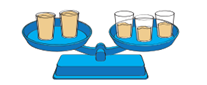
\includegraphics[scale=0.8]{img/problemas2x2_f01.png}}
\end{problem}
\begin{solution}
Seja $x$ a massa, em gramas, de um copo vazio e seja $y$ a massa, em gramas, que está dentro de um copo cheio de farinha.
Do enunciado temos que
$$\left\{ \begin{array}{ccc}
2x + 2y              & = & 3x + 3\ \dfrac{y}{2} \\[12pt]
2x + 3\ \dfrac{y}{2}  & = & 1400 \end{array}    \right.$$
Resolvendo esse sistema obtemos $x=200$ e $y=400$. Portanto um copo vazio tem o peso de 200 gramas.
\end{solution}

% Exercício 3
\begin{problem}
Oito vasos iguais, encaixados, formam uma pilha de $36\ cm$ de altura, como na figura. Dezesseis vasos iguais aos primeiros, também encaixados, formam outra pilha de $60\ cm$ de altura. Qual é a altura de cada vaso?

\centerline{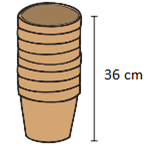
\includegraphics[scale=0.8]{img/problemas2x2_f02.png}}
\end{problem}
\begin{solution}
Vamos dividir cada vaso em duas partes: a parte de baixo de altura $x$ e a parte de cima (borda superior) de altura $y$, ou seja, a altura de cada vaso é $x+y$. A altura da pilha de oito vasos é $x+8y=36$ e a altura da pilha de dezesseis vasos é $x+16y=90$. Daí obtemos o sistema
$$\left\{ \begin{array}{rrrrr}
x   & + &   8y  &   = &  36 \\
x   & + &  16y  &   = &  90 \end{array} \right.$$
A solução desse sistema é $x=12$ e $y=3$. A altura de um vaso é $x+y=12+3=15\ cm$.
\end{solution}

% Exercício 4
\begin{problem}
Uma treinadora de basquete aplica o seguinte sistema de pontuação em seus treinos de arremesso à cesta: cada jogadora recebe 5 pontos por arremesso acertado e perde 2 pontos por arremesso errado. Ao fim de 50 arremessos, uma das jogadoras contabilizou 124 pontos. Qual é a diferença entre as quantidades de arremessos acertados e errados dessa jogadora?
\end{problem}
\begin{solution}
Sejam $a$ o número de acertos e seja $e$ o número de erros. Dos dados do problema podemos montar as equações
$$\left\{ \begin{array}{rrrrr}
 a   & + &   e  &   = &  50 \\
5a   & - &  2e  &   = & 124 \end{array} \right.$$
Resolvendo esse sistema obtemos $a=32$ e $e=18$.
Assim a diferença entre o número de acertos e o de erros é igual a $a-e=32-18=24$.
\end{solution}

% Exercício 5
\begin{problem}
Uma companhia de seguros levantou dados sobre os carros de determinada cidade e constatou que são roubados, em média, 150 carros por ano.
O número de carros roubados da marca X é o dobro do número de carros roubados da marca Y,
e as marcas X e Y juntas respondem por 60\% dos carros roubados. Qual é o número de carros roubados da marca Y por ano ?
\end{problem}
\begin{solution}
Vamos representar por $x$ o número de carros roubados da marca X e vamos representar por $y$ o número de carros roubados da marca Y por ano.
Do enunciado, podemos escrever as equações
$$\left\{ \begin{array}{rcl}
 x       & = &   2y \\[10pt]
 x + y   & = &  \dfrac{60}{100} \cdot 150 = 90\end{array} \right.$$

Resolvendo obtemos $x=60$ e $y=30$. Assim, 30 carros da marca Y são roubados por ano.
\end{solution}

% Exercício 6
\begin{problem}
Em uma festa com $n$ pessoas, em um dado instante, 31 mulheres se retiraram e restaram convidados na razão de 2 homens para cada mulher. Um pouco mais tarde, 55 homens se retiraram e restaram, a seguir, convidados na razão de 3 mulheres para cada homem. Determine o número $n$ de pessoas presentes inicialmente na festa.
\end{problem}
\begin{solution}
Suponhamos que no início da festa estavam presentes $h$ homens e $m$ mulheres. A tabela a seguir resume os dados do enunciado.

\begin{center}
\begin{tabular}{|c|c|c|c|} \hline
                             & Quantidade de homens    & Quantidade de mulheres    &  Equação          \\ \hline
Após saída de 31 mulheres    &        $h$              &    $m-31$                 &  $h=2(m-31)$      \\ \hline
 Após saída de 55 homens     &      $h-55$             &    $m-31$                 &  $m-31=3(h-55)$   \\ \hline
\end{tabular}
\end{center}

Daí obtemos o sistema linear
$$\left\{ \begin{array}{ccc}
h     & = &  2(m-31)   \\[5pt]
m-31  & = &  3(h-55)   \end{array} \right.$$
Resolvendo esse sistema obtemos $h=66$ e $m=64$. Assim o número total de pessoas na festa era de $n=h+m=66+64=130$.
\end{solution}

% Exercício 7
\begin{problem}
Em uma festa o número de mulheres era quatro vezes o número de homens.
Após a chegada de cinco casais, a porcentagem de homens na festa passou a ser 26\%.
\begin{enumerate}
\item[(a)] Qual era o percentual de homens na festa antes da chegada dos cinco casais?
\item[(b)] Quantos homens e quantas mulheres a festa passou a ter depois da chegada dos cinco casais?
\end{enumerate}
\end{problem}
\begin{solution}
\begin{enumerate}
\item[(a)] Seja $m$ o número de mulheres e seja $h$ o número de homens antes da chegada dos cinco casais.
Como o número de mulheres era quatro vezes o número dos homens, temos $m=4h$.
Deste modo, a fração de homens antes da chegada dos cinco casais era
$$\dfrac{h}{m+h} = \dfrac{h}{4h+h} = \dfrac{h}{5h} = \dfrac{1}{5} = 20\% $$
Logo o percentual de homens na festa antes da chegada dos cinco casais era 20\%.

\item[(b)] Após a chegada dos 5 casais, o número de homens passou a ser $h+5$ e o número de mulheres $m+5$.
A fração de homens na festa passou a ser então
$$\dfrac{h+5}{(m+5)+(h+5)} = \dfrac{h+5}{4h+5+h+5} = \dfrac{h+5}{5h+10}$$
Como a porcentagem de homens na festa passou a ser de 26\%, temos a equação 
$$\dfrac{h+5}{5h+10} = \dfrac{26}{100} = \dfrac{13}{50}$$
Resolvendo essa equação obtemos $h=8$. Daí obtemos $m=4h=32$.
Logo haviam $h+5=13$ homens e $m+5=37$ mulheres na festa depois da chegada dos cinco casais.
\end{enumerate}
\end{solution}

% Exercício 8
\begin{problem}
Durante uma festa de colégio, um grupo de alunos organizou uma rifa. Oitenta alunos faltaram à festa e não participaram da rifa.
Entre os que compareceram, alguns compraram três bilhetes, 45 compraram 2 bilhetes, e muitos compraram apenas um.
O total de alunos que comprou um único bilhete era 20\% do número total de bilhetes vendidos, e o total de bilhetes vendidos excedeu em 33 o número total de alunos do colégio. Quantos alunos compraram somente um bilhete?
\end{problem}
\begin{solution}
Seja $x$ a quantidade de alunos que comprou 1 bilhete e seja $y$ a quantidade de alunos que comprou 3 bilhetes.
Então temos que 80 alunos não compraram a rifa, $x$ alunos compraram um bilhete, 45 alunos compraram dois bilhetes e $y$ alunos compraram três bilhetes. Como nenhum aluno comprou quatro ou mais bilhetes podemos concluir que a quantidade de alunos do colégio é igual a soma
$80+x+45+y = x+y+125$. Já a quantidade total de bilhetes vendidos no colégio é igual a 

$$0 \cdot 80  +  1 \cdot x  +  2 \cdot 45  +  3 \cdot y = x+3y+90 $$

Segundo o enunciado, podemos montar as equações

$$\left\{ \begin{array}{ccc}
x        & = &  0,2 \, (x+3y+90)  \\[5pt]
x+3y+90  & = & (x+y+125) + 33  \end{array}\right.$$

Resolvendo o sistema encontramos $x=48$ e $y=34$. Portanto 48 alunos compraram apenas um bilhete da rifa.
\end{solution}

% Exercício 9
\begin{problem}
Em uma classe com 14 alunos, 8 são mulheres e 6 são homens. A média das notas das mulheres no final do semestre ficou 1 ponto acima da média da classe. A soma das notas dos homens foi metade da soma das notas das mulheres. Qual foi a média das notas dos homens?
\end{problem}
\begin{solution}
Seja $x$ a soma das notas das 8 mulheres e seja $y$ a soma das notas dos 6 homens.
A média das notas das mulheres é $x/8$, a média das notas dos homens é $y/6$ e a média de todos os alunos é $(x+y)/14$.
As afirmações do enunciado podem ser resumidas no seguinte sistema linear.
$$\left\{ \begin{array}{ccc}
\dfrac{x}{8}    & = &    \dfrac{x+y}{14} + 1   \\[10pt]
y               & = &    \dfrac{x}{2}           \end{array}\right.$$
Resolvendo esse sistema obtemos $x=56$ e $y=28$. A média das notas dos homens foi de $y/6 = 28/6 = 14/3 \simeq 4,66$.
\end{solution}

% Exercício 10
\begin{problem}
Ao longo de uma estrada reta estão localizadas, nessa ordem, as cidades A, B, C e D. A respeito da distância entre essas cidades sabe-se que:
\begin{itemize}
\item A distância de B até D é igual a dois terços da distância de B até A.
\item A cidade C está a 210 km da cidade A e a cidade C está 20 km mais próxima de D do que de B.
\end{itemize}

\begin{enumerate} 
\item[(a)] Represente por $x$ a distância entre A e B e represente por $y$ a distância entre B e C. Modele matematicamente o problema e relacione as variáveis $x$ e $y$ em termos de um sistema com duas equações lineares.
\item[(b)] Resolva esse sistema e, em seguida, calcule as distâncias entre as cidades C e D.
\end{enumerate}
\end{problem}
\begin{solution}
\begin{enumerate}
\item[(a)] Se $x$ é a distância entre as cidades A e B e se $y$ é a distância entre as cidades B e C, então a distância entre as cidades B e D é $2x/3$ e a distância entre as cidades C e D é $y-20$, conforme ilustrado a seguir.

\centerline{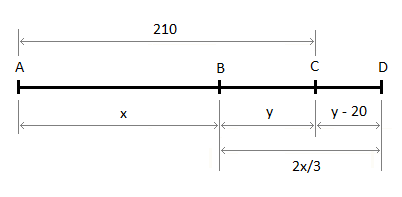
\includegraphics[scale=0.8]{img/problemas2x2_f03.png}}

A distância entre as cidades A e C é $x+y=210$. A distância entre as cidades B e D é $y+(y-20)=2x/3$.
Com essas duas equações podemos escrever o sistema de equações lineares.
$$\left\{ \begin{array}{ccc}
x+y        & = &   210     \\[5pt]
y+(y-20)   & = &   2x/3    \end{array}\right.$$
Escrevendo do modo usual, esse sistema tem o seguinte aspecto.
$$\left\{ \begin{array}{rrrrr}
            x   & + &   y  &   = &  210 \\[6pt]
\dfrac{2}{3}x   & - &  2y  &   = &  -20 \end{array} \right.$$

\item[(b)] Para resolver o sistema linear do item anterior podemos multiplicar a primeira equação por 2 para obter
$$\left\{ \begin{array}{rrrrr}
           2x   & + &  2y  &   = &  420 \\[6pt]
\dfrac{2}{3}x   & - &  2y  &   = &  -20 \end{array} \right.$$
Somando essas duas equações obtemos 
$$\dfrac{8x}{3} = 400$$
A solução dessa equação é $x=150$. Substituindo na primeira equação do sistema obtemos $150+y=210$ cuja solução é $y=60$.
Portanto a solução do sistema é $x=150$ e $y=60$. Desse modo as distâncias entre as cidades são:

\begin{itemize}
\item Distância entre A e B: $x=150$ km.
\item Distância entre B e C: $y=60$ km.
\item Distância entre C e D: $y-20=40$ km.
\end{itemize}
\end{enumerate}
\end{solution}
